\documentclass[11pt,a4paper]{article}

% ── Packages ──────────────────────────────────────────────
\usepackage[margin=2cm, headheight=14pt]{geometry}
\usepackage{amsmath}
\usepackage{booktabs}
\usepackage{array}
\usepackage{xcolor}
\usepackage{colortbl}
\usepackage{multirow}
\usepackage{tikz}
\usetikzlibrary{arrows.meta, patterns}
\usepackage{pgfplots}
\usepgfplotslibrary{fillbetween}
\pgfplotsset{compat=1.18}
\usepackage{siunitx}
\usepackage{enumitem}
\usepackage{fancyhdr}
\usepackage{hyperref}

% ── Colours ───────────────────────────────────────────────
\definecolor{hdrblue}{HTML}{2C3E50}
\definecolor{rowgray}{HTML}{F2F2F2}
\definecolor{accentred}{HTML}{E74C3C}
\definecolor{accentgreen}{HTML}{27AE60}
\definecolor{accentorange}{HTML}{F39C12}
\definecolor{accentpurple}{HTML}{8E44AD}
\definecolor{lightblue}{HTML}{EBF5FB}

% ── Header / Footer ──────────────────────────────────────
\pagestyle{fancy}
\fancyhf{}
\lhead{\textcolor{hdrblue}{\textbf{SAFEFL --- VM Requirements (Medium Models)}}}
\rhead{\textcolor{hdrblue}{\today}}
\cfoot{\thepage}

% ── Macros ────────────────────────────────────────────────
\newcommand{\gb}[1]{\SI{#1}{\giga\byte}}
\newcommand{\mb}[1]{\SI{#1}{\mega\byte}}
\newcommand{\sectionrule}{\noindent\textcolor{hdrblue}{\rule{\linewidth}{0.6pt}}\vspace{4pt}}
\newcommand{\mobnet}{MobileNetV3-S}
\newcommand{\resnet}{ResNet18}

\begin{document}

% ══════════════════════════════════════════════════════════
\begin{center}
  {\LARGE\bfseries\textcolor{hdrblue}{Cloud VM Requirements}}\\[4pt]
  {\large SAFEFL --- MobileNetV3-Small \& ResNet18}\\[2pt]
  {\small Medium-size models\,---\,Vertex\,AI\,---\,500 clients\,---\,Krum aggregation}
\end{center}
\sectionrule

% ══════════════════════════════════════════════════════════
\section*{Model Comparison}

\noindent
\begin{center}
\renewcommand{\arraystretch}{1.3}
\begin{tabular}{
  >{\raggedright\arraybackslash}p{4cm}
  >{\centering\arraybackslash}p{4.5cm}
  >{\centering\arraybackslash}p{4.5cm}}
\toprule
\rowcolor{hdrblue}
\textcolor{white}{\textbf{Property}} &
\textcolor{white}{\textbf{MobileNetV3-Small}} &
\textcolor{white}{\textbf{ResNet18}} \\
\midrule
Parameters             & $\sim$962\,K ($\sim$1.0\,M)  & $\sim$11\,200\,K ($\sim$11.2\,M) \\
\rowcolor{rowgray}
Gradient size (float32)& \mb{3.85}                    & \mb{44.8} \\
Target dataset         & FEMNIST (62 classes)          & FEMNIST (62 classes) \\
\bottomrule
\end{tabular}
\end{center}

% ══════════════════════════════════════════════════════════
\section*{Experiment Configuration}

\noindent
\begin{center}
\renewcommand{\arraystretch}{1.3}
\begin{tabular}{
  >{\raggedright\arraybackslash}p{3.8cm}
  >{\raggedright\arraybackslash}p{9.5cm}}
\toprule
\rowcolor{hdrblue}
\textcolor{white}{\textbf{Parameter}} &
\textcolor{white}{\textbf{Value}} \\
\midrule
Dataset        & FEMNIST ($1\!\times\!28\!\times\!28$, 62 classes, federated across writers) \\
\rowcolor{rowgray}
Clients        & 500 (sequential local training per round) \\
Aggregation    & Krum --- $\mathcal{O}(n^{2}\!\cdot\!d)$ pairwise distance computation \\
\rowcolor{rowgray}
Batch size     & 32 \\
\bottomrule
\end{tabular}
\end{center}

% ══════════════════════════════════════════════════════════
\section*{Memory Breakdown --- Side by Side}

\noindent
\begin{center}
\renewcommand{\arraystretch}{1.3}
\begin{tabular}{
  >{\raggedright\arraybackslash}p{5cm}
  S[table-format=2.2]
  S[table-format=2.2]
  >{\raggedright\arraybackslash}p{3.8cm}}
\toprule
\rowcolor{hdrblue}
\textcolor{white}{\textbf{Component}} &
\textcolor{white}{\textbf{\mobnet{} (GB)}} &
\textcolor{white}{\textbf{\resnet{} (GB)}} &
\textcolor{white}{\textbf{Notes}} \\
\midrule
Gradient storage ($500 \times d \times 4$\,B)
                        & 1.93   & 22.40  & Dominates for ResNet18 \\
\rowcolor{rowgray}
Model + optimizer state & 0.02   & 0.18   & Single copy on GPU \\
Training activations    & 0.25   & 1.20   & Batch\,=\,32 \\
\rowcolor{rowgray}
Dataset + OS overhead   & 1.00   & 1.00   & FEMNIST + buffers \\
\midrule
\textbf{Total system RAM}  & \textbf{3.20}  & \textbf{24.78} & \textbf{Minimum} \\
\rowcolor{rowgray}
\textbf{Recommended RAM}   & \textbf{8.00}  & \textbf{32.00} & \textbf{With safety margin} \\
\midrule
\textbf{GPU VRAM}           & \textbf{2.00}  & \textbf{4.00}  & Single GPU sufficient \\
\bottomrule
\end{tabular}
\end{center}

% ── RAM comparison bar chart ─────────────────────────────
\noindent
\begin{center}
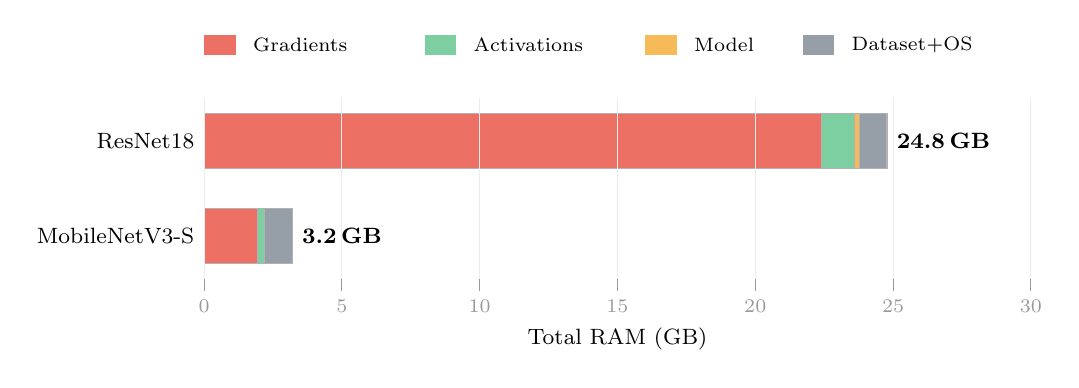
\begin{tikzpicture}
  % Two groups of stacked bars side by side
  \def\xscale{0.35}  % 1 GB = 0.35cm → 30 GB ≈ 10.5cm
  \def\barh{0.35}

  % --- MobileNetV3-Small (bottom group, y=0) ---
  \def\yM{0}
  % Gradient: 1.93 GB
  \fill[accentred!80, draw=black!30]
    (0,\yM-\barh) rectangle ({1.93*\xscale},\yM+\barh);
  % Activations: 0.25
  \fill[accentgreen!60, draw=black!30]
    ({1.93*\xscale},\yM-\barh) rectangle ({(1.93+0.25)*\xscale},\yM+\barh);
  % Model: 0.02
  \fill[accentorange!70, draw=black!30]
    ({(1.93+0.25)*\xscale},\yM-\barh) rectangle ({(1.93+0.25+0.02)*\xscale},\yM+\barh);
  % Dataset+OS: 1.00
  \fill[hdrblue!50, draw=black!30]
    ({(1.93+0.25+0.02)*\xscale},\yM-\barh) rectangle ({(1.93+0.25+0.02+1.00)*\xscale},\yM+\barh);
  % Label
  \node[right, font=\footnotesize\bfseries] at ({3.20*\xscale},\yM) {3.2\,GB};
  \node[left, font=\footnotesize] at (0,\yM) {MobileNetV3-S};

  % --- ResNet18 (top group, y=1.2) ---
  \def\yR{1.2}
  % Gradient: 22.40 GB
  \fill[accentred!80, draw=black!30]
    (0,\yR-\barh) rectangle ({22.40*\xscale},\yR+\barh);
  % Activations: 1.20
  \fill[accentgreen!60, draw=black!30]
    ({22.40*\xscale},\yR-\barh) rectangle ({(22.40+1.20)*\xscale},\yR+\barh);
  % Model: 0.18
  \fill[accentorange!70, draw=black!30]
    ({(22.40+1.20)*\xscale},\yR-\barh) rectangle ({(22.40+1.20+0.18)*\xscale},\yR+\barh);
  % Dataset+OS: 1.00
  \fill[hdrblue!50, draw=black!30]
    ({(22.40+1.20+0.18)*\xscale},\yR-\barh) rectangle ({(22.40+1.20+0.18+1.00)*\xscale},\yR+\barh);
  % Label
  \node[right, font=\footnotesize\bfseries] at ({24.78*\xscale},\yR) {24.8\,GB};
  \node[left, font=\footnotesize] at (0,\yR) {ResNet18};

  % Axis
  \draw[black!60] (0,-0.55) -- (0,1.75);
  \foreach \v/\l in {0/0, 5/5, 10/10, 15/15, 20/20, 25/25, 30/30} {
    \draw[black!40] ({\v*\xscale},-0.55) -- ({\v*\xscale},-0.7)
      node[below, font=\scriptsize] {\l};
    \draw[gray!15] ({\v*\xscale},-0.55) -- ({\v*\xscale},1.75);
  }
  \node[below, font=\footnotesize] at ({15*\xscale},-1.05) {Total RAM (GB)};

  % Legend
  \fill[accentred!80] (0,2.3) rectangle (0.4,2.55);
  \node[right, font=\scriptsize] at (0.5,2.425) {Gradients};
  \fill[accentgreen!60] (2.8,2.3) rectangle (3.2,2.55);
  \node[right, font=\scriptsize] at (3.3,2.425) {Activations};
  \fill[accentorange!70] (5.6,2.3) rectangle (6.0,2.55);
  \node[right, font=\scriptsize] at (6.1,2.425) {Model};
  \fill[hdrblue!50] (7.6,2.3) rectangle (8.0,2.55);
  \node[right, font=\scriptsize] at (8.1,2.425) {Dataset+OS};

\end{tikzpicture}
\par\medskip{\small\textcolor{hdrblue}{\textbf{Stacked RAM breakdown}} --- ResNet18 requires $\sim$8$\times$ more memory than MobileNetV3-Small.}
\end{center}

% ══════════════════════════════════════════════════════════
\section*{Vertex AI VM Options}

\noindent
\begin{center}
\renewcommand{\arraystretch}{1.35}
\begin{tabular}{
  >{\raggedright\arraybackslash}p{3.5cm}
  c c c
  >{\centering\arraybackslash}p{2cm}
  >{\centering\arraybackslash}p{2cm}}
\toprule
\rowcolor{hdrblue}
\textcolor{white}{\textbf{Machine Type}} &
\textcolor{white}{\textbf{GPUs}} &
\textcolor{white}{\textbf{vCPUs}} &
\textcolor{white}{\textbf{RAM}} &
\textcolor{white}{\textbf{\mobnet{}}} &
\textcolor{white}{\textbf{\resnet{}}} \\
\midrule
\texttt{n1-standard-4} + T4
  & 1$\times$T4\,16G & 4  & \gb{15}
  & \textcolor{accentgreen}{\textbf{Safe}}
  & \textcolor{accentred}{\textbf{OOM}} \\
\rowcolor{rowgray}
\texttt{n1-standard-8} + T4
  & 1$\times$T4\,16G & 8  & \gb{30}
  & \textcolor{accentgreen}{\textbf{Safe}}
  & \textcolor{accentorange}{\textbf{Tight}} \\
\texttt{n1-highmem-8} + T4
  & 1$\times$T4\,16G & 8  & \gb{52}
  & \textcolor{accentgreen}{\textbf{Safe}}
  & \textcolor{accentgreen}{\textbf{Safe}} \\
\rowcolor{rowgray}
\texttt{n1-standard-16} + V100
  & 1$\times$V100\,16G & 16  & \gb{60}
  & \textcolor{accentgreen}{\textbf{Safe}}
  & \textcolor{accentgreen}{\textbf{Safe}} \\
\texttt{a2-highgpu-1g}
  & 1$\times$A100\,40G & 12  & \gb{85}
  & \textcolor{accentgreen}{\textbf{Safe}}
  & \textcolor{accentgreen}{\textbf{Safe}} \\
\bottomrule
\end{tabular}
\end{center}

% ══════════════════════════════════════════════════════════
\section*{Runtime Estimates (per Round, 500 Clients)}

\noindent
\begin{center}
\renewcommand{\arraystretch}{1.3}
\begin{tabular}{
  >{\raggedright\arraybackslash}p{5cm}
  >{\centering\arraybackslash}p{2.5cm}
  >{\centering\arraybackslash}p{2.5cm}
  >{\raggedright\arraybackslash}p{3.5cm}}
\toprule
\rowcolor{hdrblue}
\textcolor{white}{\textbf{Phase}} &
\textcolor{white}{\textbf{\mobnet{}}} &
\textcolor{white}{\textbf{\resnet{}}} &
\textcolor{white}{\textbf{Complexity}} \\
\midrule
Local training (500 clients)  & 1--2\,min & 3--5\,min & $\mathcal{O}(n \cdot B \cdot d)$ \\
\rowcolor{rowgray}
Krum aggregation               & 5--15\,s  & 1--3\,min & $\mathcal{O}(n^{2}\!\cdot\!d)$ \\
Model update + logging         & $<$5\,s   & $<$10\,s  & $\mathcal{O}(d)$ \\
\midrule
\textbf{Total per round}       & \textbf{1--3\,min} & \textbf{4--8\,min} & \\
\rowcolor{rowgray}
\textbf{100 rounds}            & \textbf{2--5\,hrs} & \textbf{7--14\,hrs} & \\
\bottomrule
\end{tabular}
\end{center}

% ══════════════════════════════════════════════════════════
\section*{Aggregation Cost at $n=500$ (Krum)}

\noindent
\begin{center}
\renewcommand{\arraystretch}{1.3}
\begin{tabular}{
  >{\raggedright\arraybackslash}p{4cm}
  >{\centering\arraybackslash}p{4cm}
  >{\centering\arraybackslash}p{4cm}}
\toprule
\rowcolor{hdrblue}
\textcolor{white}{\textbf{Metric}} &
\textcolor{white}{\textbf{MobileNetV3-Small}} &
\textcolor{white}{\textbf{ResNet18}} \\
\midrule
Gradient dimension $d$    & 962\,000       & 11\,200\,000 \\
\rowcolor{rowgray}
Pairwise pairs $\binom{500}{2}$ & 124\,750 & 124\,750 \\
FLOPs per round (Krum)    & $\sim$240\,B   & $\sim$2\,800\,B \\
\rowcolor{rowgray}
FLOPs per round (FedAvg)  & $\sim$0.48\,B  & $\sim$5.6\,B \\
Krum / FedAvg ratio       & $500\times$    & $500\times$ \\
\bottomrule
\end{tabular}
\end{center}

% ── Scaling figure (same shape, different d) ─────────────
\noindent
\begin{center}
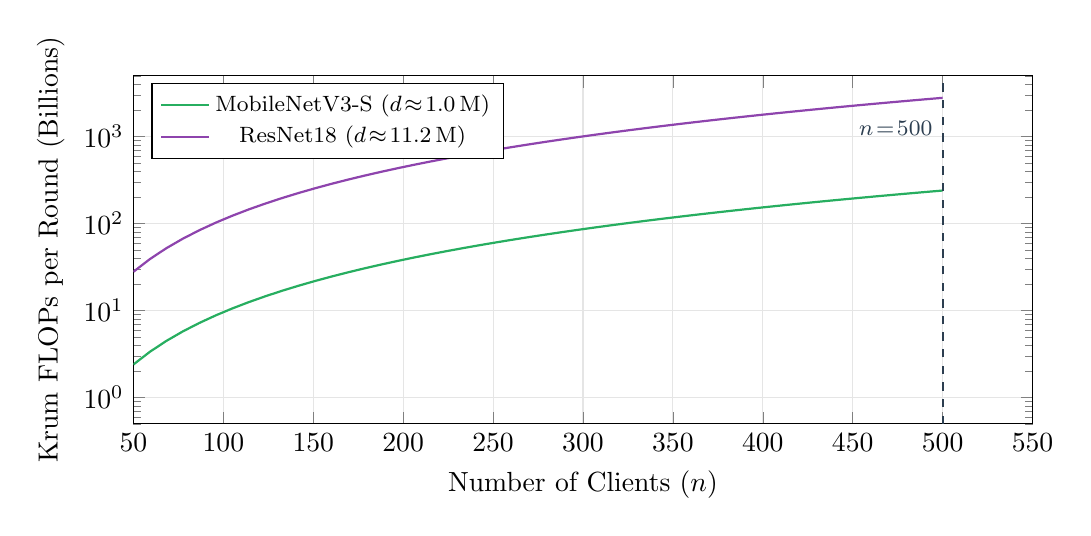
\begin{tikzpicture}
  \begin{axis}[
    width=13cm, height=6cm,
    xlabel={Number of Clients ($n$)},
    ylabel={Krum FLOPs per Round (Billions)},
    ymode=log,
    xmin=50, xmax=550,
    ymin=0.5, ymax=5000,
    legend style={at={(0.02,0.98)}, anchor=north west, font=\footnotesize},
    grid=major,
    grid style={gray!20},
    every axis plot/.append style={thick},
  ]
  % MobileNetV3: d≈962000, Krum FLOPs = n^2 * d
  \addplot[accentgreen, mark=none, domain=50:500, samples=50]
    {(x^2) * 962000 / 1e9};
  \addlegendentry{MobileNetV3-S ($d\!\approx\!1.0$\,M)}

  % ResNet18: d≈11200000, Krum FLOPs = n^2 * d
  \addplot[accentpurple, mark=none, domain=50:500, samples=50]
    {(x^2) * 11200000 / 1e9};
  \addlegendentry{ResNet18 ($d\!\approx\!11.2$\,M)}

  % Vertical line at 500
  \draw[hdrblue, dashed, thick] (axis cs:500,0.5) -- (axis cs:500,5000)
    node[pos=0.85, left, font=\footnotesize\bfseries, text=hdrblue] {$n\!=\!500$};
  \end{axis}
\end{tikzpicture}
\par\medskip{\small\textcolor{hdrblue}{\textbf{Krum aggregation cost}} --- both scale as $\mathcal{O}(n^{2})$; ResNet18 is $\sim$11.4$\times$ more expensive per round.}
\end{center}

% ══════════════════════════════════════════════════════════
\section*{Recommendation}

\noindent
\begin{center}
\renewcommand{\arraystretch}{1.4}
\begin{tabular}{
  >{\raggedright\arraybackslash}p{3cm}
  >{\raggedright\arraybackslash}p{5cm}
  >{\raggedright\arraybackslash}p{5cm}}
\toprule
\rowcolor{hdrblue}
\textcolor{white}{\textbf{}} &
\textcolor{white}{\textbf{MobileNetV3-Small}} &
\textcolor{white}{\textbf{ResNet18}} \\
\midrule
Machine   & \texttt{n1-standard-4} + T4       & \texttt{n1-highmem-8} + T4 \\
\rowcolor{rowgray}
RAM       & \gb{15}                            & \gb{52} \\
GPU       & 1$\times$T4 16\,GB                 & 1$\times$T4 16\,GB \\
\rowcolor{rowgray}
vCPUs     & 4                                  & 8 \\
Disk      & 200\,GB SSD                        & 200\,GB SSD \\
\bottomrule
\end{tabular}
\end{center}

% ══════════════════════════════════════════════════════════
\section*{Comparison with ViT-B-16 (Worst Case)}

\noindent
\begin{center}
\renewcommand{\arraystretch}{1.3}
\begin{tabular}{
  >{\raggedright\arraybackslash}p{3.5cm}
  >{\centering\arraybackslash}p{3cm}
  >{\centering\arraybackslash}p{3cm}
  >{\centering\arraybackslash}p{3cm}}
\toprule
\rowcolor{hdrblue}
\textcolor{white}{\textbf{Metric}} &
\textcolor{white}{\textbf{MobileNetV3-S}} &
\textcolor{white}{\textbf{ResNet18}} &
\textcolor{white}{\textbf{ViT-B-16}} \\
\midrule
Parameters              & 1.0\,M     & 11.2\,M    & 85.8\,M \\
\rowcolor{rowgray}
Gradient (500 clients)  & 1.9\,GB    & 22.4\,GB   & 171.5\,GB \\
Total RAM needed        & $\sim$3\,GB& $\sim$25\,GB & $\sim$220\,GB \\
\rowcolor{rowgray}
GPU VRAM needed         & 2\,GB      & 4\,GB      & 24\,GB \\
Krum FLOPs/rnd          & 240\,B     & 2\,800\,B  & 21\,450\,B \\
\rowcolor{rowgray}
Time per 100 rnds       & 2--5\,hrs  & 7--14\,hrs & 25--42\,hrs \\
Min.\ VM tier           & T4 + 8\,GB  & T4 + 32\,GB & A100 + 256\,GB \\
\bottomrule
\end{tabular}
\end{center}

% ══════════════════════════════════════════════════════════
\section*{Notes}

\noindent
\begin{center}
\renewcommand{\arraystretch}{1.25}
\begin{tabular}{
  >{\centering\arraybackslash}p{0.6cm}
  >{\raggedright\arraybackslash}p{13cm}}
\toprule
\rowcolor{hdrblue}
\textcolor{white}{\textbf{\#}} &
\textcolor{white}{\textbf{Note}} \\
\midrule
1 & FEMNIST is naturally federated (partitioned by writer); non-IID by default. \\
\rowcolor{rowgray}
2 & MobileNetV3-Small fits comfortably on a single T4 GPU (\gb{16} VRAM). \\
3 & ResNet18 with 500 clients needs $\sim$25\,GB RAM --- a standard \texttt{n1-standard-8} (\gb{30}) is tight but feasible. \\
\rowcolor{rowgray}
4 & FactorGraphs with grouping ($k \leq 15$) reduces aggregation memory from $\mathcal{O}(n^{2})$ to $\mathcal{O}(g^{2})$. \\
\bottomrule
\end{tabular}
\end{center}

\end{document}
